%!TEX root = ./template-skripsi.tex
%-------------------------------------------------------------------------------
%                            BAB III
%               		PEMBAHASAN
%-------------------------------------------------------------------------------

\chapter{PEMBAHASAN}

\section{Rancangan Algoritma}
Pada pembuatan steganografi dengan metode LSB ini menggunakan bantuan MATLAB. Dan citra \emph{digital} yang digunakan adalah dengan format BMP, alasan dipilihnya citra dengan format BMP adalah karena kesesuaiannya dengan metode LSB. Dan pesan yang disisipkan adalah pesan dengan format \emph{text}

	\subsection{Proses Penyisipan (\emph{Encoding}) pesan ke Citra \emph{Digital}}
	Proses penyisipan pesan ke citra yaitu:
	\begin{enumerate}
		\item Siapkan \emph{Cover Image} yang akan disisipkan \emph{Hiddentext}
		\item Masukkan \emph{Hiddentext} yang akan disisipkan
		\item \emph{Cover Image} dikonversi setiap nilai \emph{pixel}-nya ke biner, sedangkan \emph{Hiddentext} dikonversi dari huruf ke ASCII dan dikonversi lagi menjadi biner
		\item Proses \emph{Encoding} dilakukan dengan LSB
		\item Selanjutnya proses konversi dari biner ke \emph{pixel} yang menghasilkan \emph{Stego Image}
		\item Hasil dari citra yang telah disisipkan pesan atau \emph{Stego Image} disimpan
	\end{enumerate}
	
	\begin{figure}[H]
		\centering
		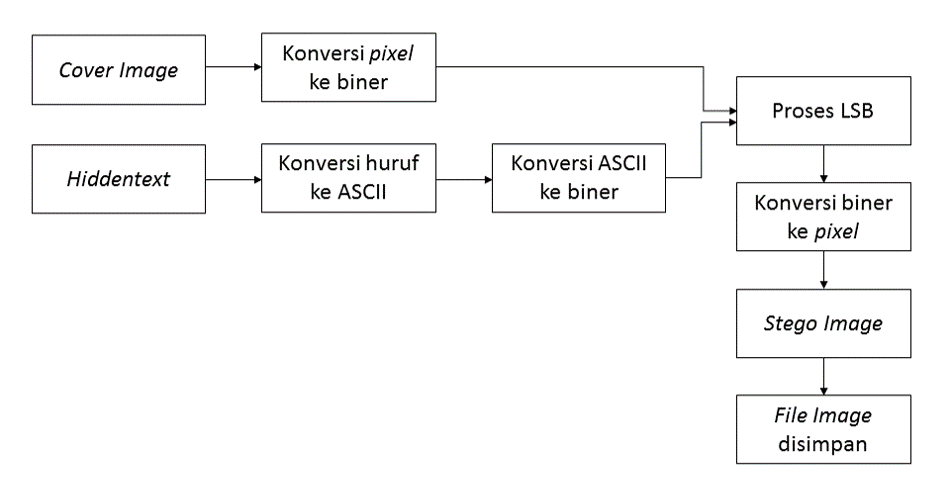
\includegraphics[width=1\textwidth]{gambar/penyisipan2}
		\caption{\emph{Flowchart} Penyisipan Pesan Rahasia}
		\label{flowchart_penyisipan}
	\end{figure}
	
	\subsection{Proses Ekstraksi (\emph{Decoding}) pesan dari Citra \emph{Digital}}
	Proses ekstraksi pesan dari citra yaitu:
	\begin{enumerate}
		\item Siapkan \emph{Stego Image} yang telah disisipkan \emph{Hiddentext}
		\item Konversi \emph{pixel} ke biner
		\item Proses \emph{Decoding} dilakukan dengan LSB
		\item Konversi biner ke \emph{pixel} untuk mendapatkan \emph{Cover Image}, dan konversi biner ke ASCII kemudian ke huruf untuk mendapatkan pesan rahasia atau \emph{Hiddentext}
		\item \emph{Hiddentext} didapatkan
	\end{enumerate}
	
	\begin{figure}[H]
		\centering
		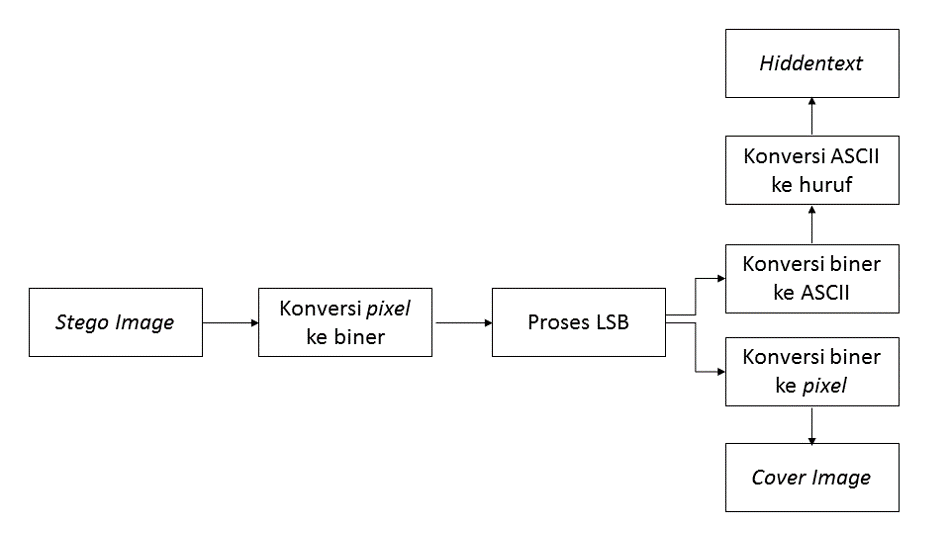
\includegraphics[width=1\textwidth]{gambar/ekstraksi2}
		\caption{\emph{Flowchart} Ekstraksi Pesan Rahasia}
		\label{flowchart_ekstraksi}
	\end{figure}
	
\section{Desain Antar Muka Program}
\section{Perbedaan Citra Sebelum dan Sesudah disisipkan Pesan}
